
\subsection*{Histogram Analysis}
Histogram plots of the retrieved well data indicate that well depth values consistently follow a lognormal distribution. The years 1920 through 2023 are divided into 5-year bins (with the exception of the 2020 to 2023 bin, which spans 4 years), and each bin demonstrates lognormal distribution clearly with an initially low concentration of well points of very shallow depth that quickly gives way to the highest concentration of points at low to mid-level depths, and then slowly tails off upon reaching deeper depths. Reinforcing this, even when histograms are restricted to 1-year periods, the lognormal trend is just as apparent (Figure~\ref{fig:OG_1yr_LN}). 
\begin{figure}[h]
    \centering
    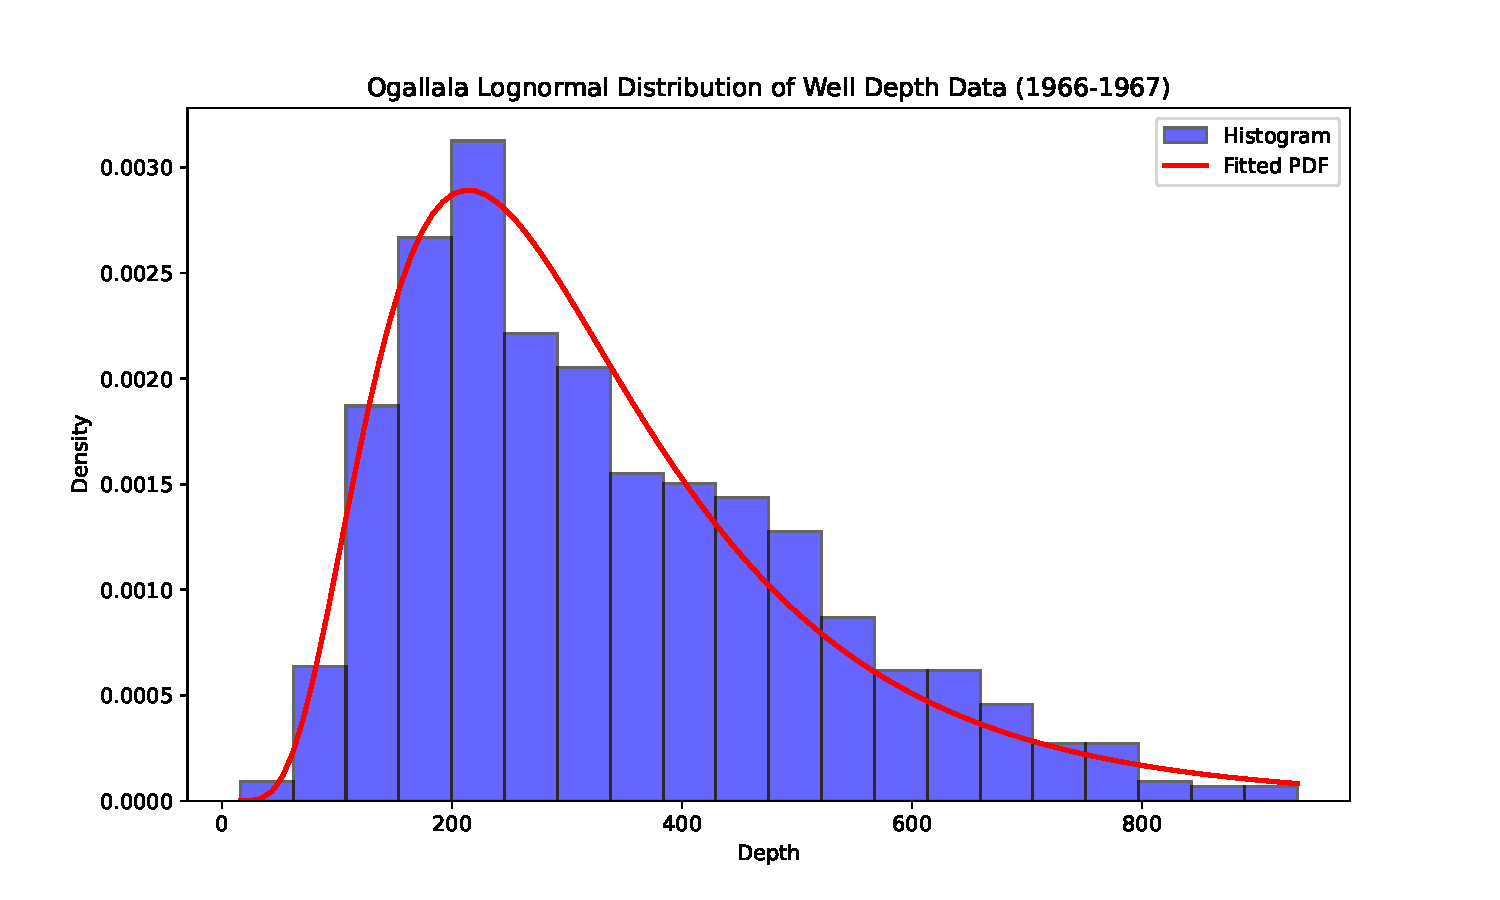
\includegraphics[width=0.5\linewidth]{Figures:Tables/Ogallala/Ogallala_LNDist_66to67.pdf}
    \caption{Enter Caption}
    \label{fig:OG_1yr_LN}
\end{figure}

\subsubsection*{Ogallala}
The data pertaining to the Ogallala aquifer has been defined by light-blue color shown in Figure~\ref{fig:OG_Histo}. Upon examining changes to the Ogallala histogram through the years, the density of well depth points depicts a deepening shift that can be observed through the increasing density deeper well depth values, as evidenced by the broadening of the red bars in more recent time bins. Associated with this trend is the increasing standard deviation values in Table OG, which suggest an increasing spread in well depth with time.

\begin{figure}[H]
    \centering
    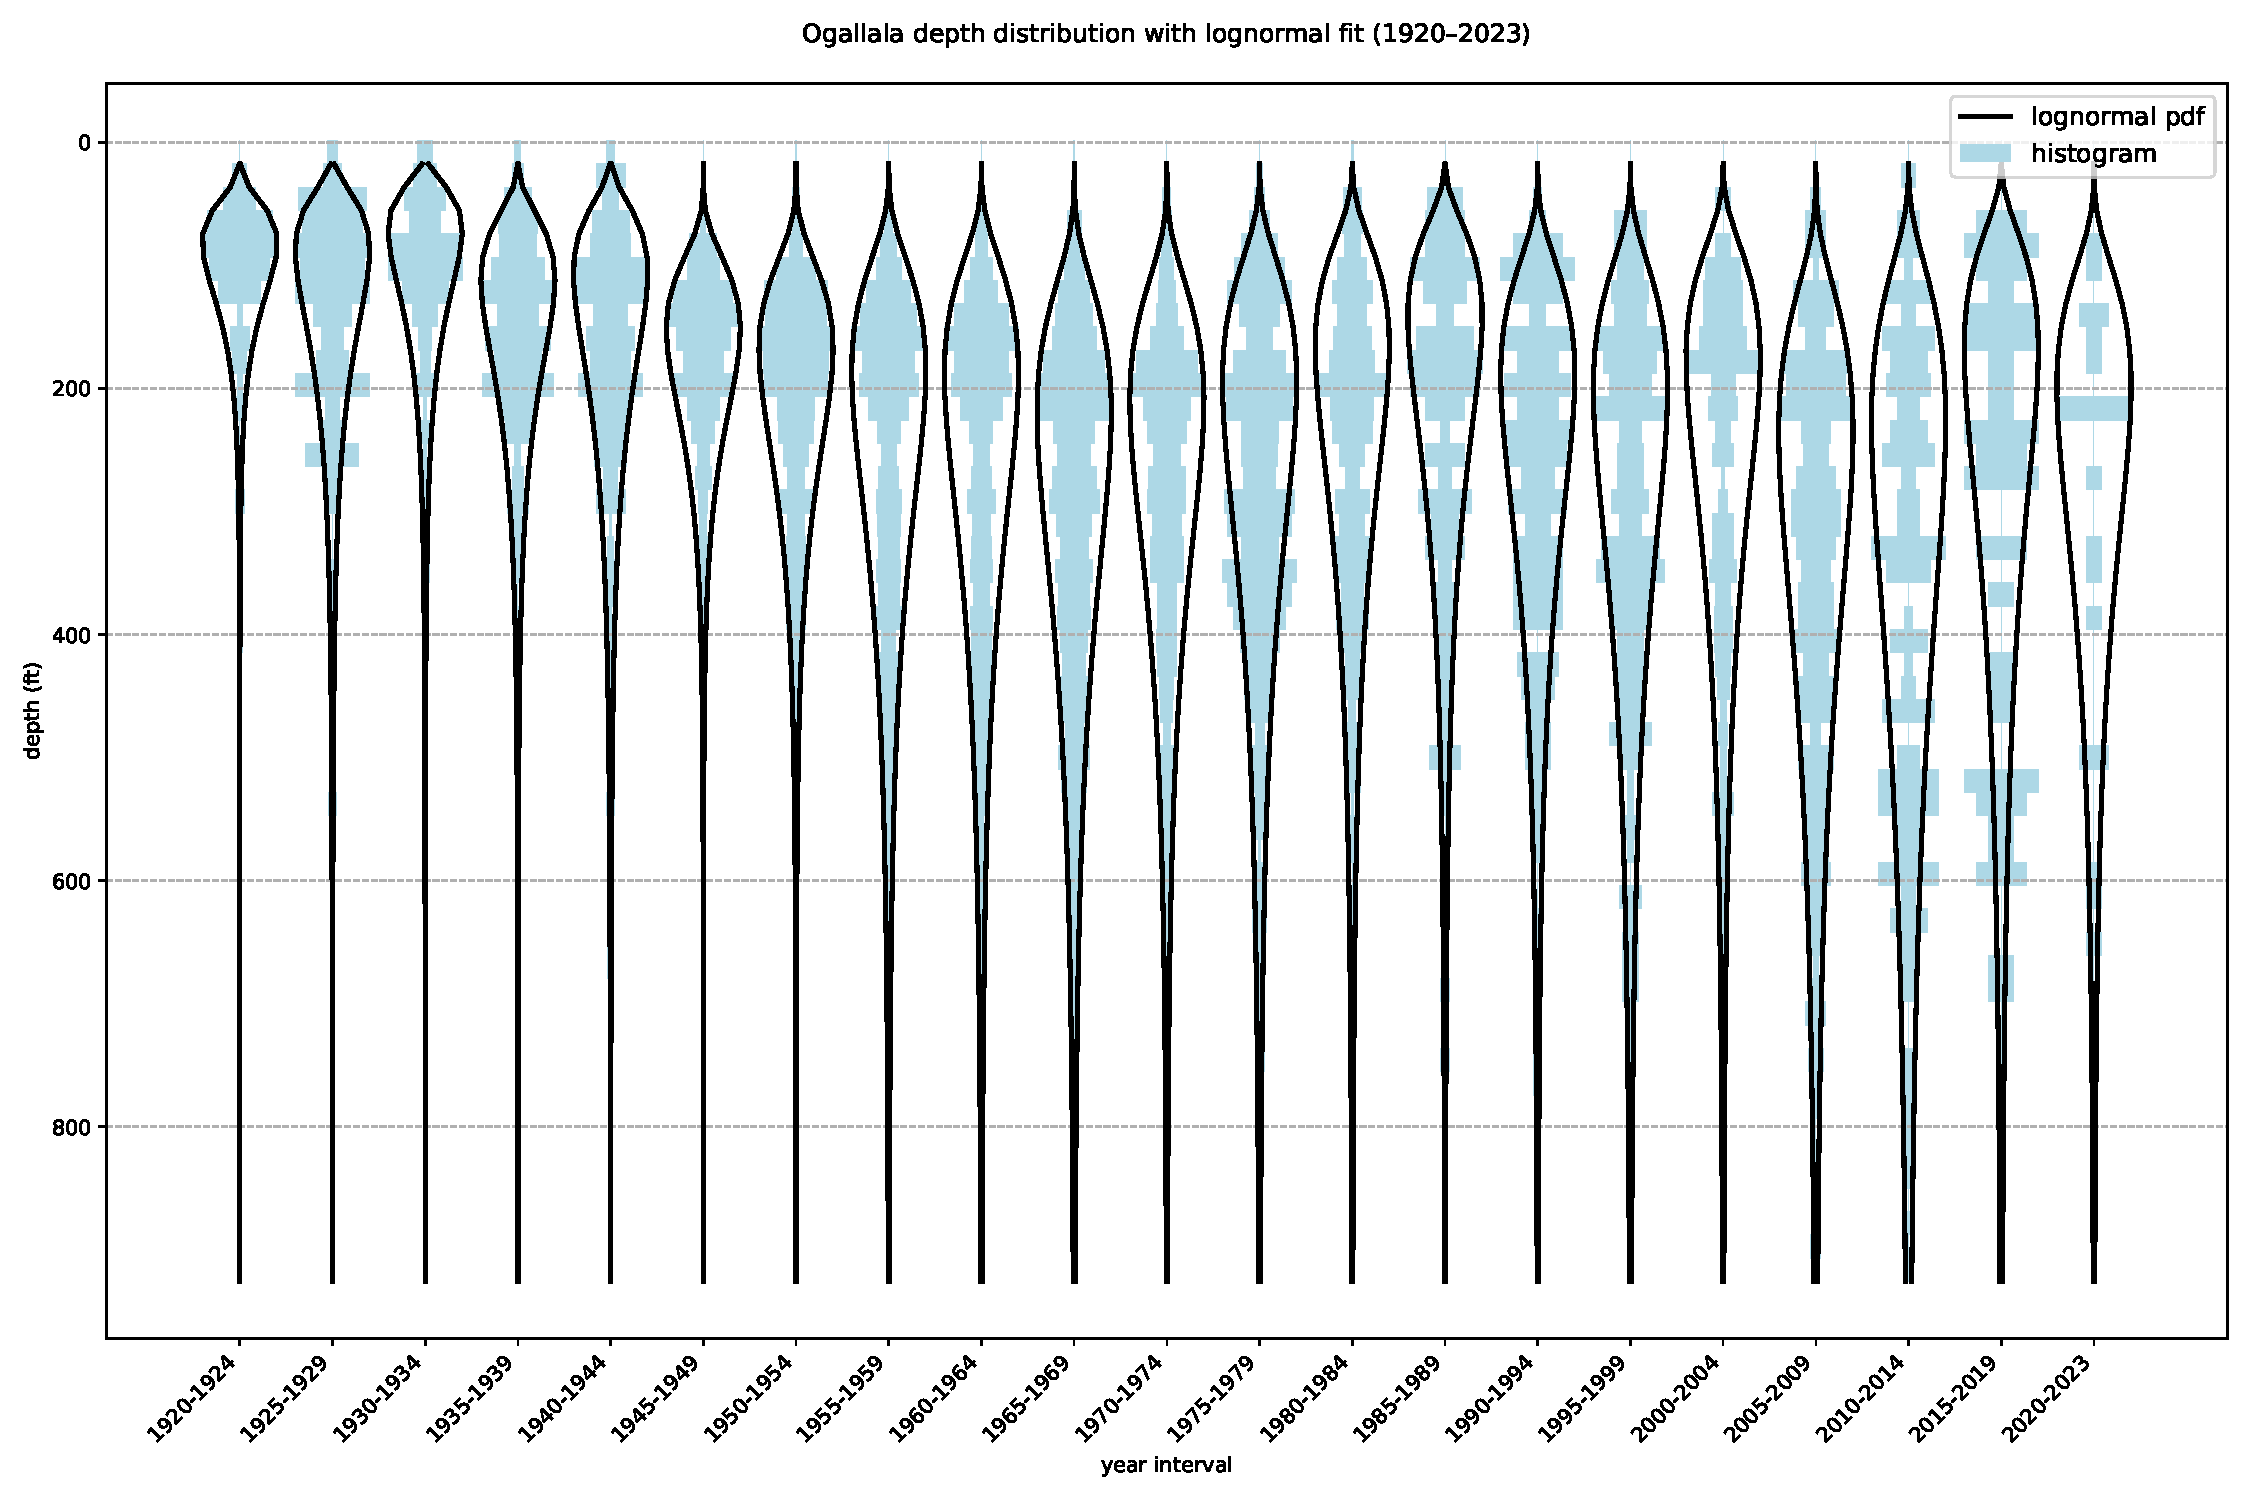
\includegraphics[width=0.5\linewidth]{Figures:Tables/Ogallala/Ogallala_histogram.pdf}
    \caption{Enter Caption}
    \label{fig:OG_Histo}
\end{figure}

\subsubsection*{Edwards (Balcones Fault Zone)}
In the Edwards (Balcones Fault Zone) Aquifer, histograms display a lognormal distribution just as in the Ogallala aquifer, but density patterns differ as the years progress. Beginning in 1920, deeper wells become increasingly common, however, this trend reverses around 1970, with shallower wells becoming more prevalent (Figure~\ref{fig:EBFZ_Histo}). Through the supplementation of Table EBFZ, it can be seen that these well points are dispersed over a large range as the lognormal standard deviation values are high.

\begin{figure}[H]
    \centering
    \includegraphics[width=0.5\linewidth]{Figures:Tables/EdwardsBFZ/EdwardsBFZ_Histo.pdf}
    \caption{Enter Caption}
    \label{fig:EBFZ_Histo}
\end{figure}

\subsubsection*{Edwards-Trinity Plateau}
Similar to the previous two aquifers, the Edwards-Trinity Plateau Aquifer exhibits lognormal distributions when grouped into 5-year bins (Figure~\ref{fig:ETP_Histo}). The density distribution of the well depths, however, remains relatively constant until the 1990s, where the distribution sees a deeper shift and data points become sparser. 

\begin{figure}[H]
    \centering
    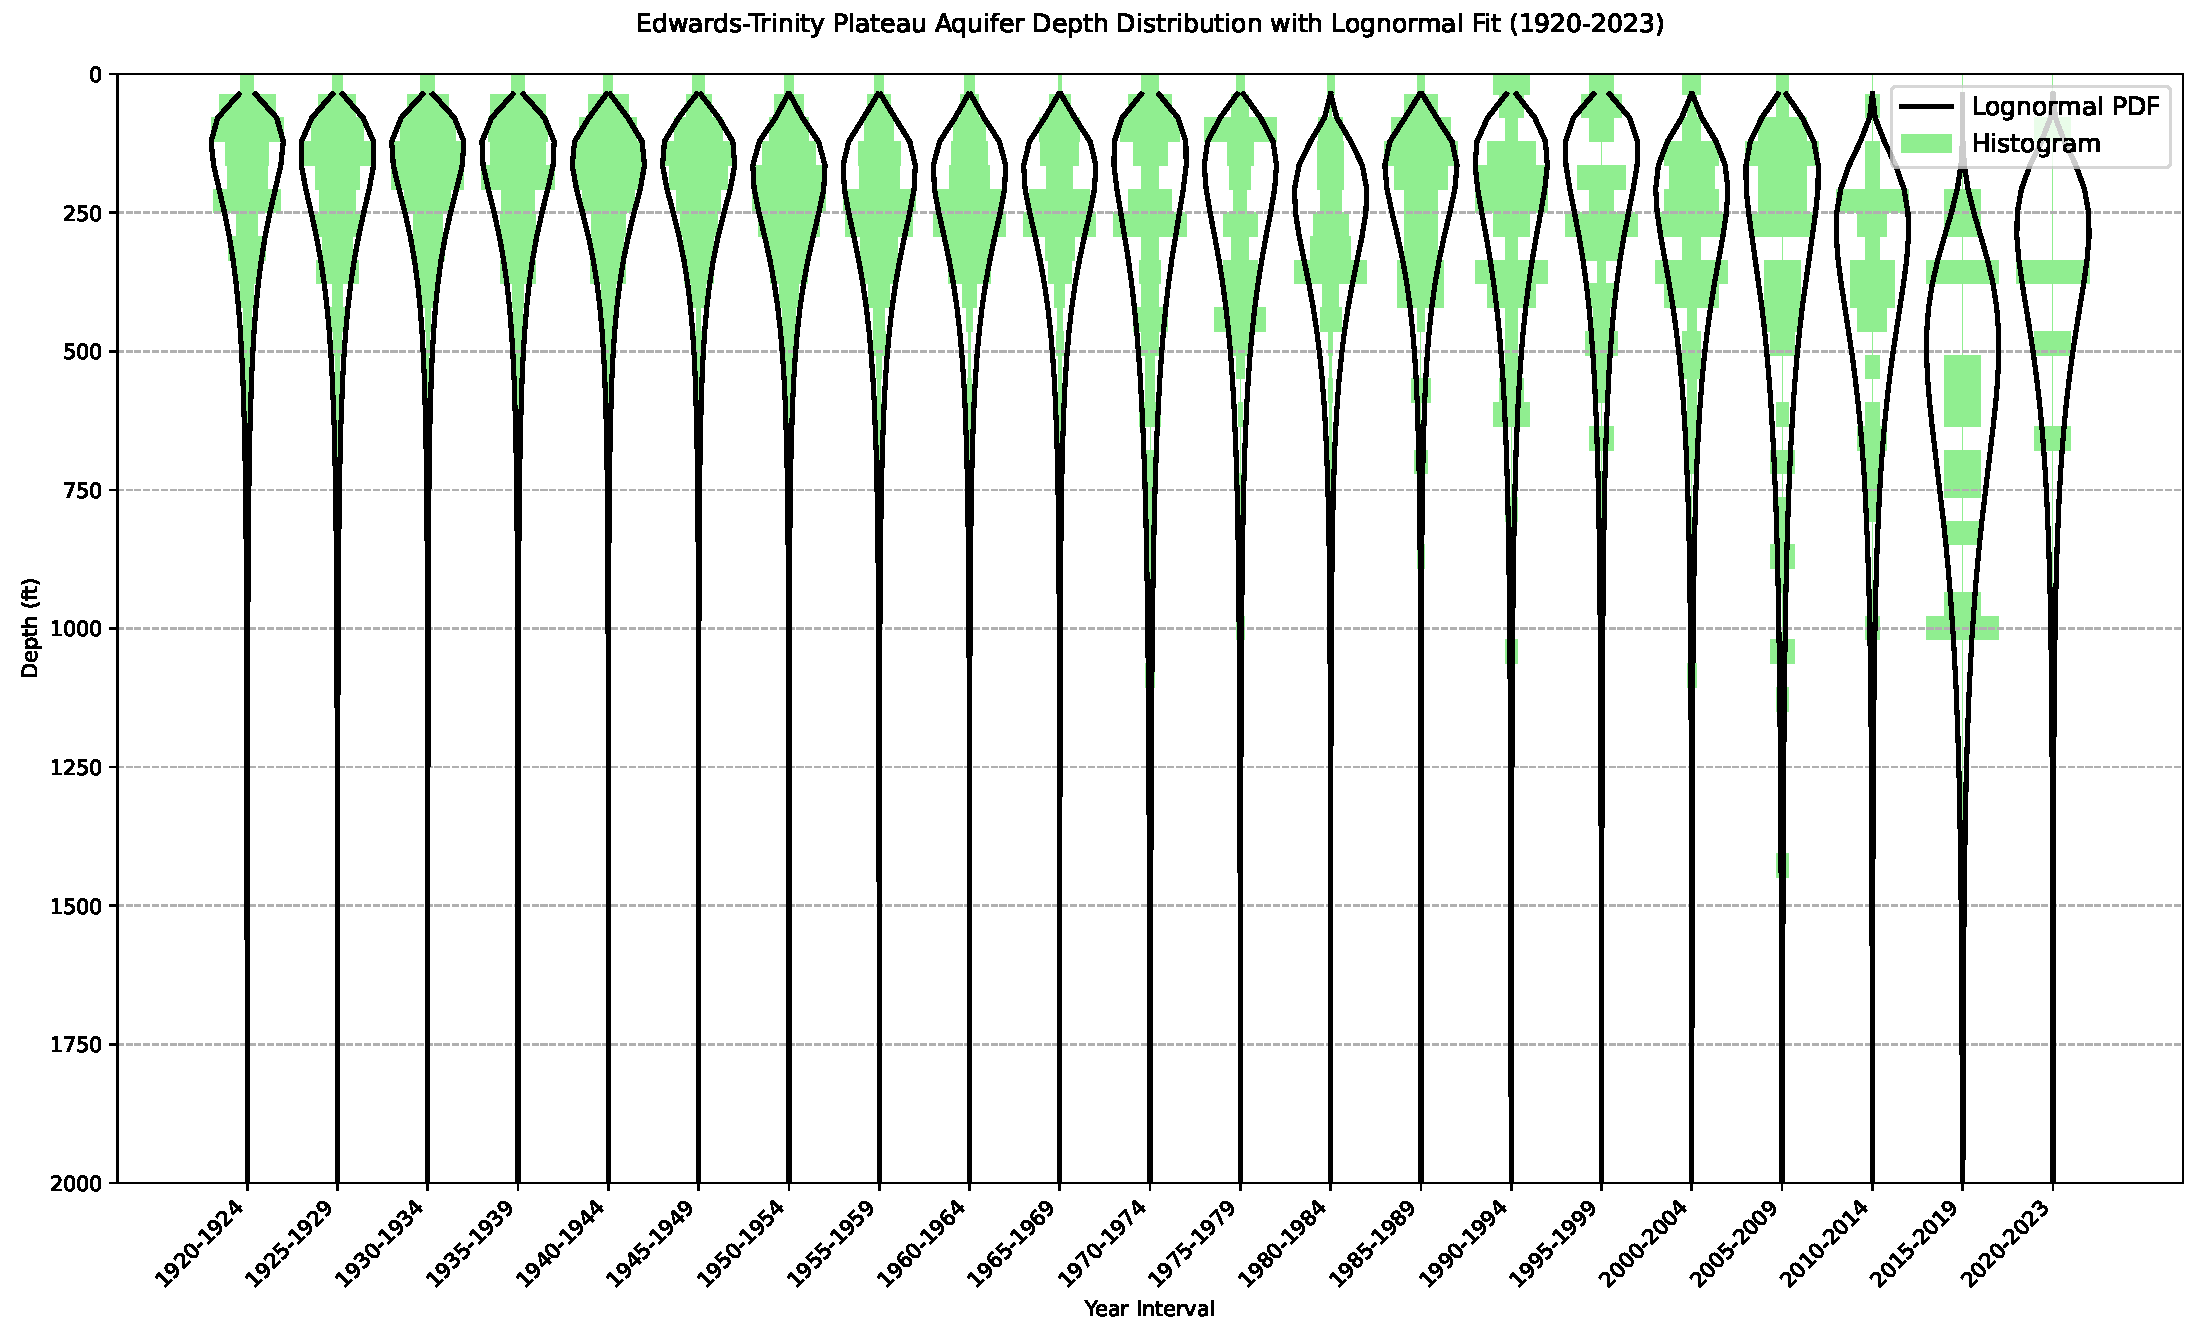
\includegraphics[width=0.5\linewidth]{Sections/Results/Results Figures:Tables/EdwardsTP/EdwardsTP_Histo.pdf}
    \caption{Enter Caption}
    \label{fig:ETP_Histo}
\end{figure}

\subsubsection*{Carrizo-Wilcox}
In the first two decades of the histogram analysis for the Carrizo-Wilcox aquifer, histograms portray a distribution that is not quite lognormal (Figure~\ref{fig:CW_Histo}). As time progresses, the distribution of depth values deepens and becomes more lognormal. The number of wells drilled per year reaches its maximum in the 1960s (Figure~\ref{fig:CW_n_value}) but even as wells drilled per year begins to decrease, the depth of wells drilled continues to increase (Figure 5).

\begin{figure}[H]
    \centering
    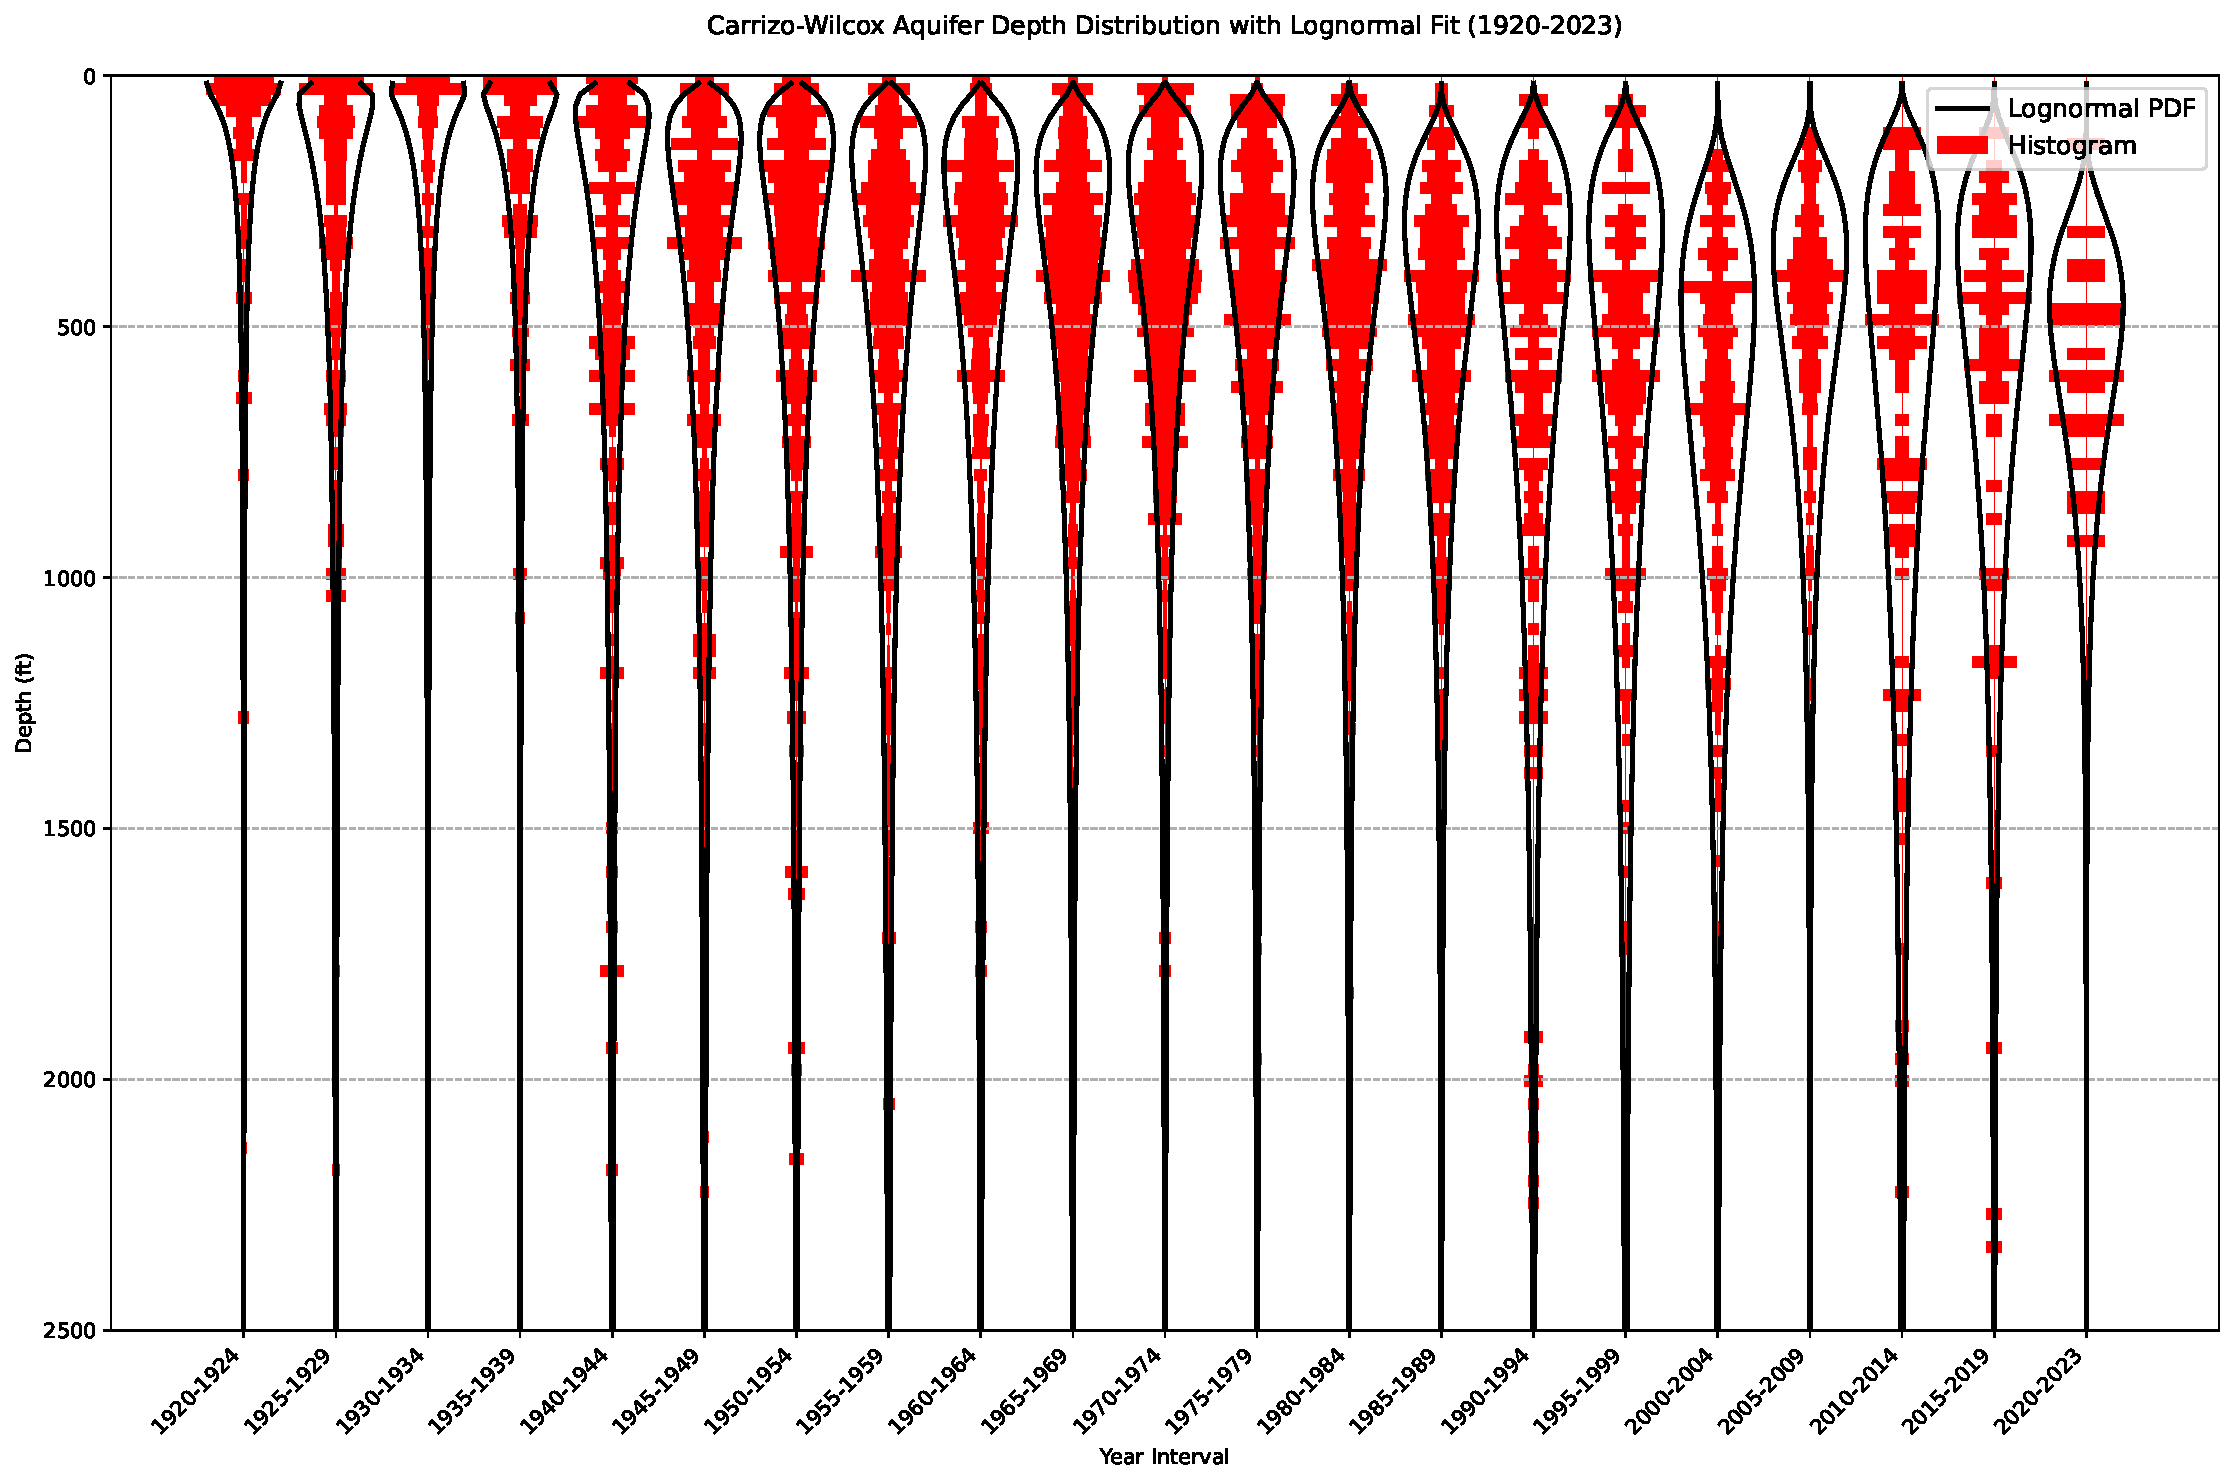
\includegraphics[width=0.5\linewidth]{Sections/Results/Results Figures:Tables/Carrizo_Wilcox/Carrizo-Wilcox_Aquifer_Depth_Distribution.pdf}
    \caption{Enter Caption}
    \label{fig:CW_Histo}
\end{figure}

\subsubsection*{Gulf Coast}
The Gulf Coast Aquifer displays a lognormal distribution in every single 5-year bin subsequent to the year 1920 (Figure~\ref{fig:GC_Histo}). As time progresses, the depth distribution of aquifer points deepens until the mid 1980’s, where the depths then recede until the 2010’s, where the spread of depth values increases greatly.

\begin{figure}[H]
    \centering
    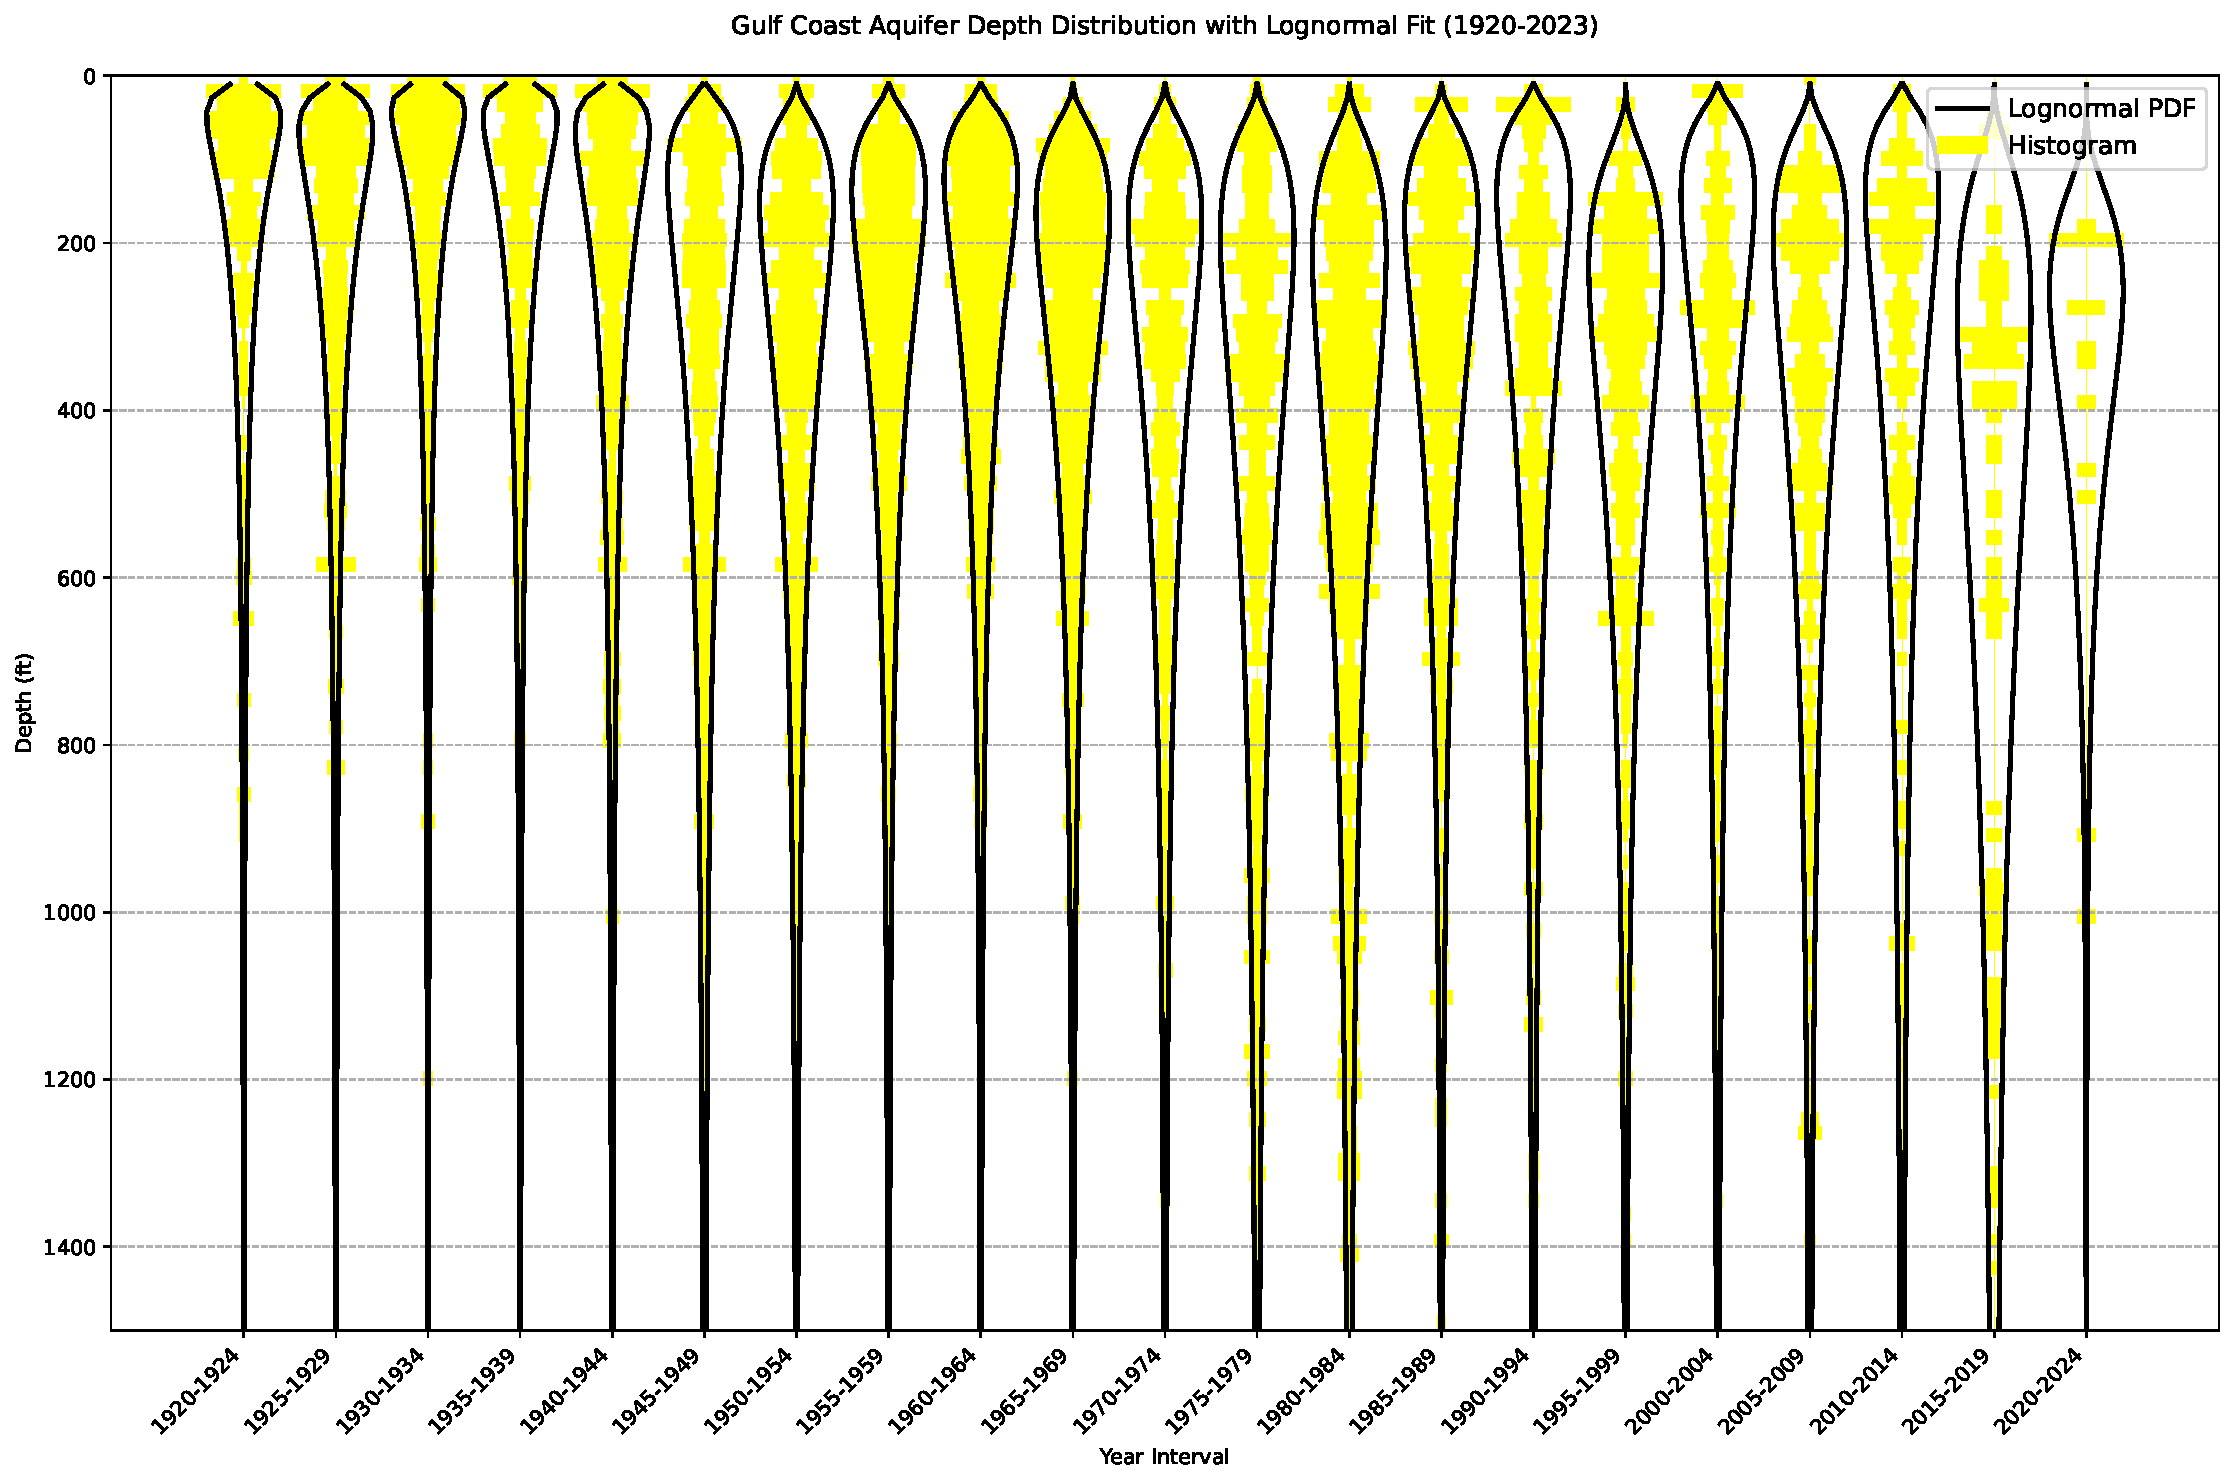
\includegraphics[width=0.5\linewidth]{Sections/Results/Results Figures:Tables/Gulf Coast/Gulf Coast_Aquifer_Depth_Distribution.pdf}
    \caption{Enter Caption}
    \label{fig:GC_Histo}
\end{figure}

\subsubsection*{Pecos Valley}
The Pecos Valley Aquifer exhibits lognormal distribution in the majority of its 5 year bins, owing the deviations from this to a lack of data (as can be seen in the year 2010-2014) (Figure~\ref{fig:PV_Histo}). The 5-year bin with the highest concentration of deep well depths is shown in 1970-1974. This time period does not see a dramatic increase in wells produced (Figure~\ref{fig:PV_n_value}). Additionally, the years 2020-2023 were unable to produce a probability density function due to a lack of values, as only one point, with a value of 702 feet, exists.


\begin{figure}[H]
    \centering
    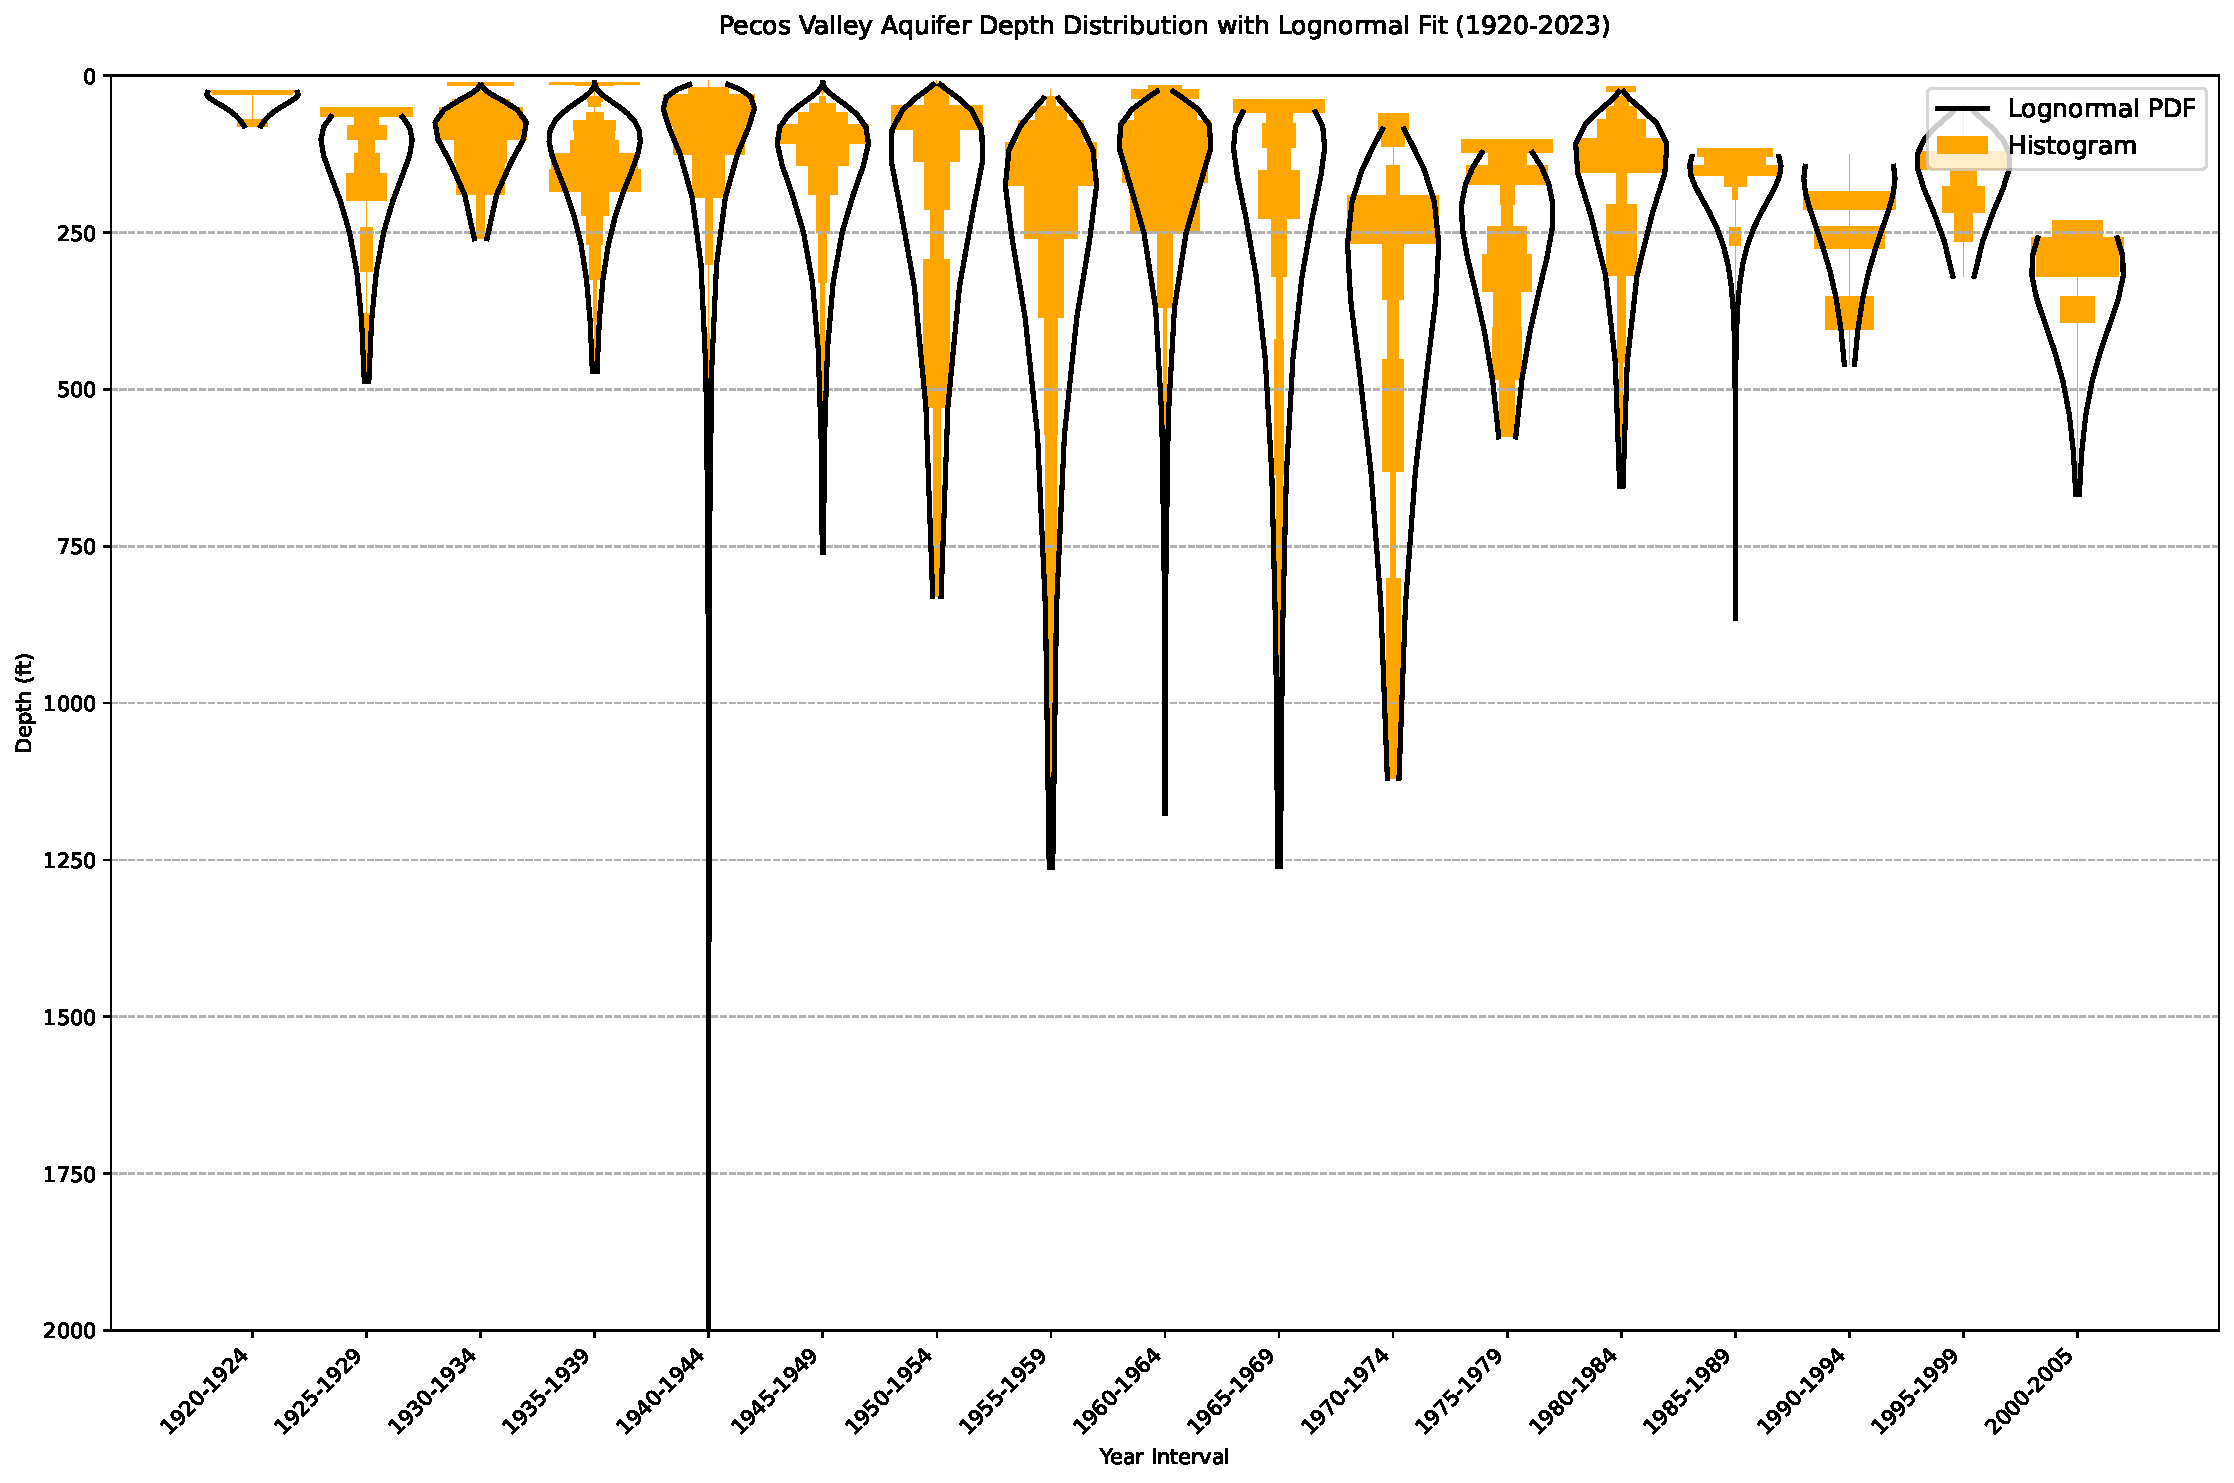
\includegraphics[width=0.5\linewidth]{Sections/Results/Results Figures:Tables/Pecos Valley/Pecos Valley_Aquifer_Depth_Distribution.pdf}
    \caption{Enter Caption}
    \label{fig:PV_Histo}
\end{figure}

\subsubsection*{Seymour}
All year bins, with the exception of the years 2010 to 2023, exhibit a lognormal distribution ~\ref{fig:SM_Histo}). Prior to the 1980’s, very little shift in the allocation of depth values can be noted, though the years after show a stretching of values downwards.

\begin{figure}[H]
    \centering
    \includegraphics[width=0.5\linewidth]{Figures:Tables/Seymour/Seymour_histogram.pdf}
    \caption{Enter Caption}
    \label{fig:SM_Histo}
\end{figure}

\subsubsection*{Trinity}
The Trinity Aquifer displays consistent lognormal distributions over the 21 5-year intervals between 1920 and 2023 and a relatively constant depth distribution (Figure~\ref{fig:TR_Histo}). The years 1965 to 1974, with emphasis on the 1965 to 1969 5-year bin, however, exhibit a deviation from the norm. These depth values display a less variable distribution, as shown by Figure~\ref{fig:TR_Histo} and the minimum std value for the total time period of 373.18 that is presented in Table TR.

\begin{figure}[H]
    \centering
    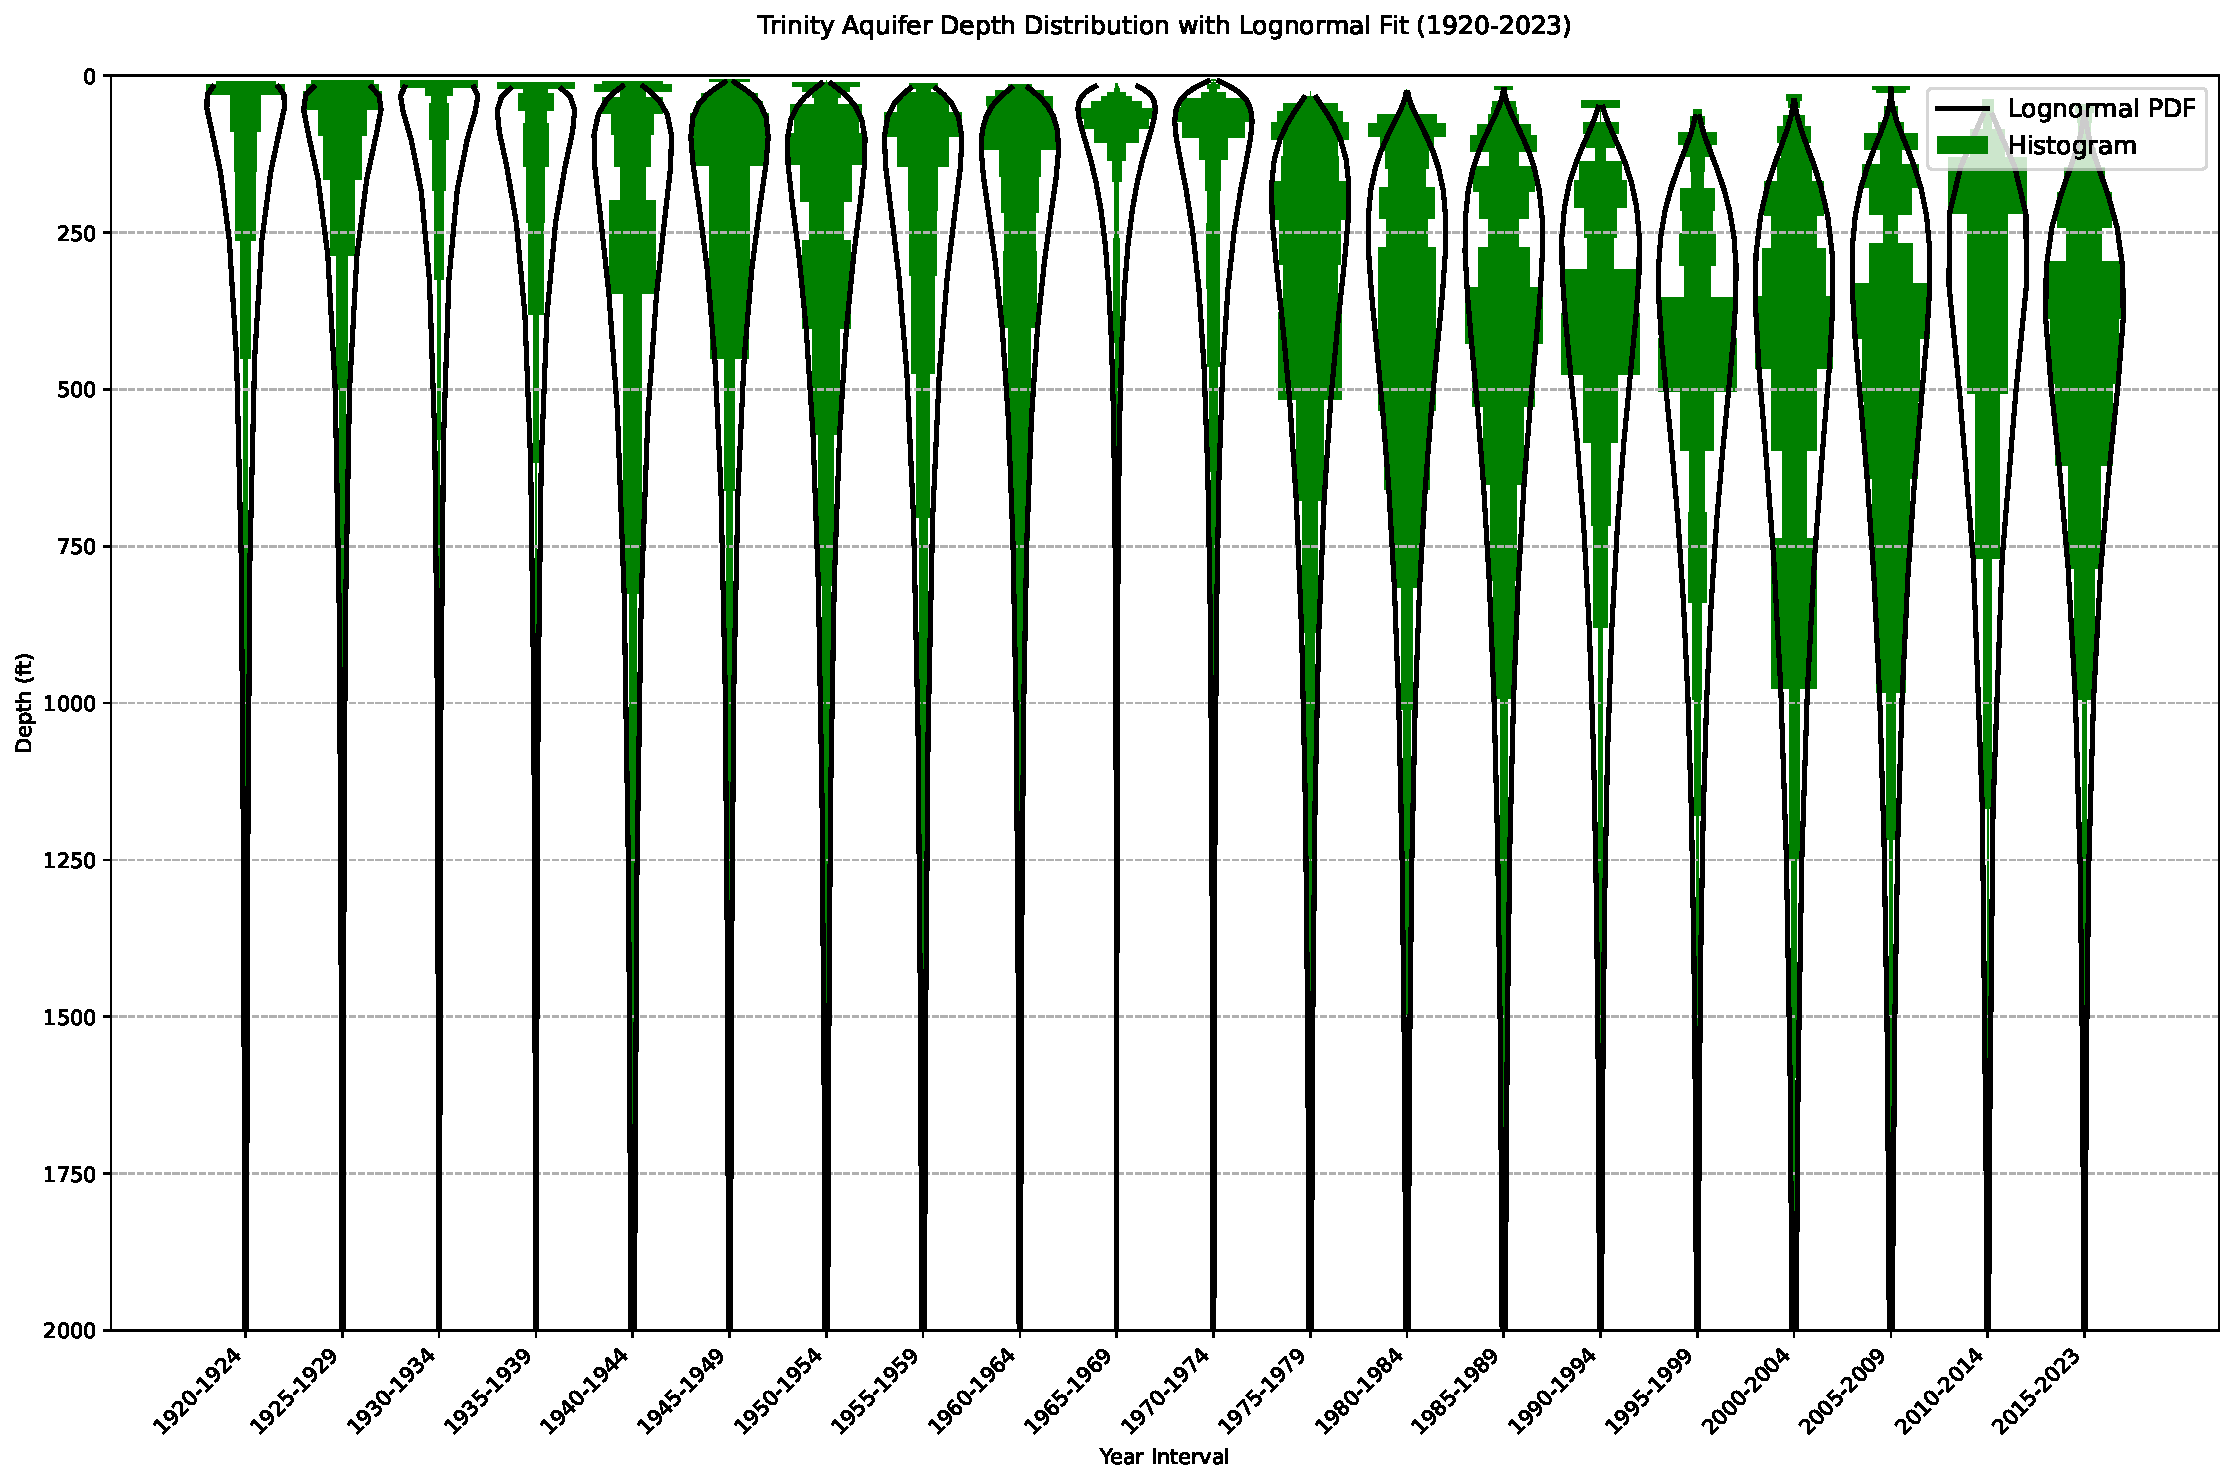
\includegraphics[width=0.5\linewidth]{Sections/Results/Results Figures:Tables/Trinity/Trinity_Aquifer_Depth_Distribution.pdf}
    \caption{Enter Caption}
    \label{fig:TR_Histo}
\end{figure}

\subsubsection*{Hueco-Mesilla Basin}
The Hueco-Mesilla Basin Aquifer, colored pink in Figure~\ref{fig:HM_Histo}, exhibits a relatively constant lognormal distribution of depths that shallow initially and then begins to expand downwards around the 1950’s, with an exception being the years 2005 to 2009 in which very little data that consisted of relatively high depth values was available (Figure~\ref{fig:HM_n_value}). 

\begin{figure}[H]
    \centering
    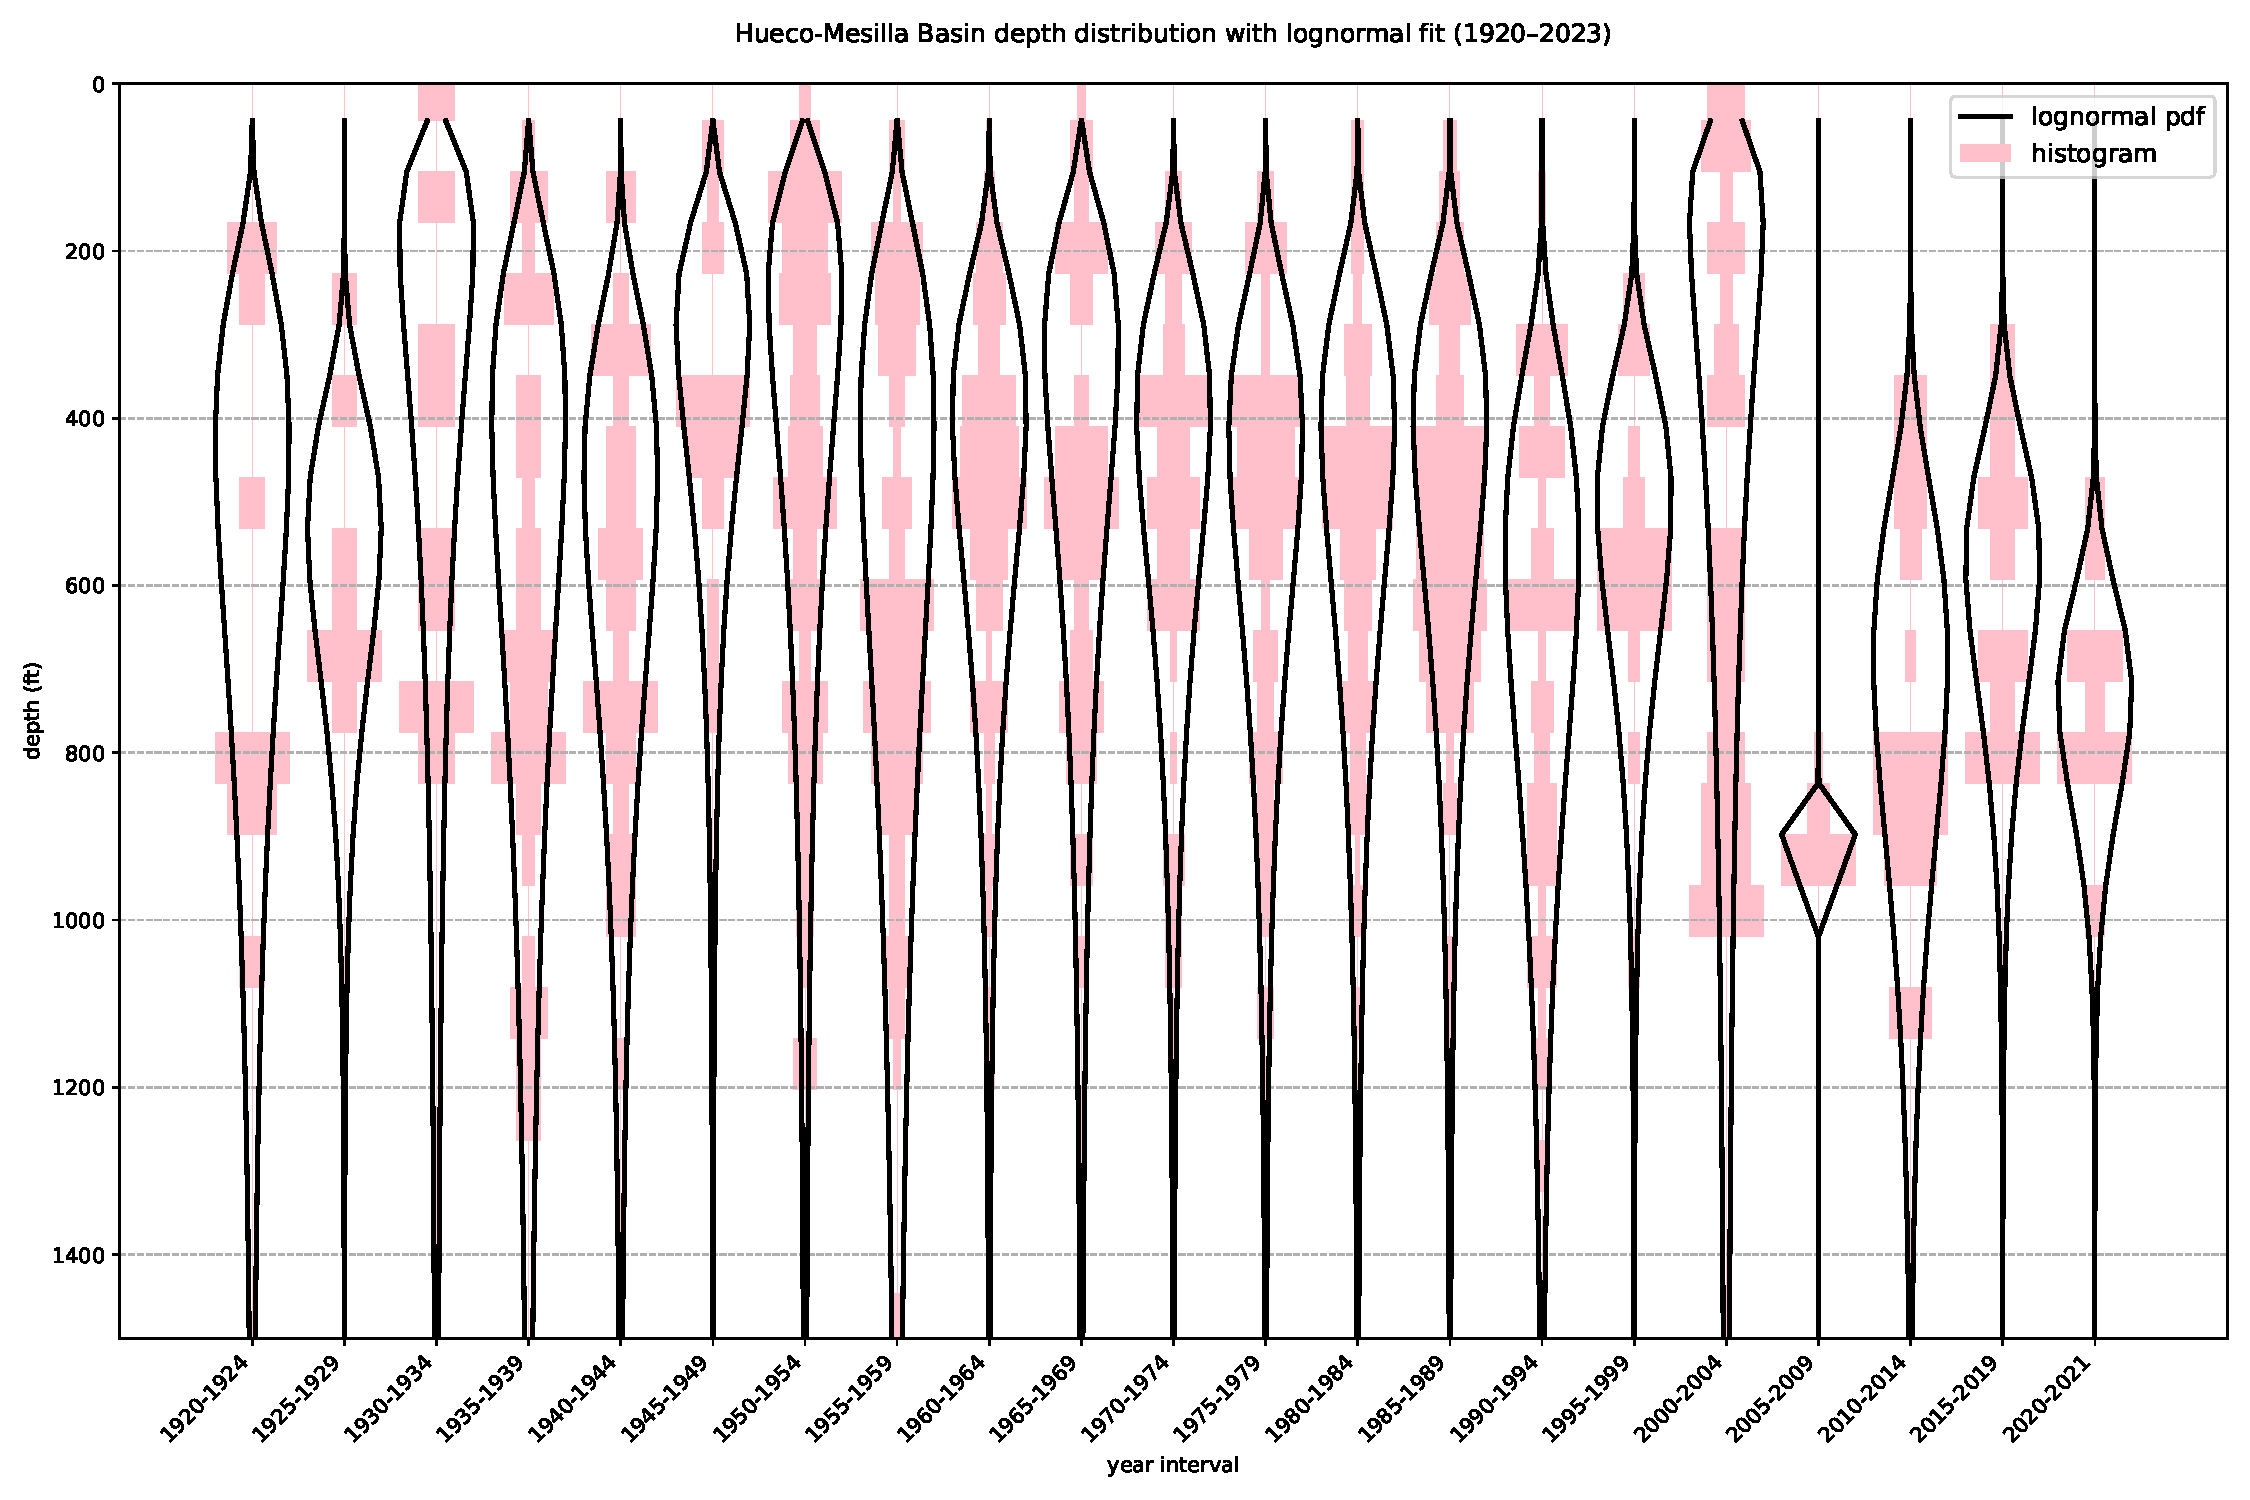
\includegraphics[width=0.5\linewidth]{Figures:Tables/Hueco-Mesilla Basin/Hueco-Mesilla_Basin_histogram.pdf}
    \caption{Enter Caption}
    \label{fig:HM_Histo}
\end{figure}
